\section{Вторая программа}
\subsection{Базовый вариант}

\begin{code}
	\captionof{listing}{Вторая программа, базовый вариант}
	\inputminted
	[
	frame=single,
	framerule=0.5pt,
	framesep=10pt,
	fontsize=\small,
	tabsize=4,
	linenos,
	numbersep=5pt,
	xleftmargin=10pt,
	]
	{c}
	{code/2_1.c}
\end{code}

\begin{figure}[!hbpt]
	\centering
	
\includegraphics[width=\textwidth]{image/2-1}
	\caption{Вывод программы}
\end{figure}

В программе один и тот же файл открывается 2 раза для чтения. При выполнении системного вызова open() создаётся дескриптор открытого файла в таблице открытых файлов процесса и запись в системной таблице открытых файлов. Так как файл открывается 2 раза, то в системной таблице открытых файлов будет создано 2 дескриптора struct file, каждый из которых имеет собственный указатель f\_pos. По этой причине чтение становится независимым --- при вызове read() для обоих дескрипторов по очереди, оба указателя проходят по всем позициям файла, и каждый символ считывается и выводится по два раза. При этом оба дескриптора struct file ссылаются на один и тот же inode.


\newpage
\subsection{Связи структур}
\begin{figure}[!h]
	\centering
	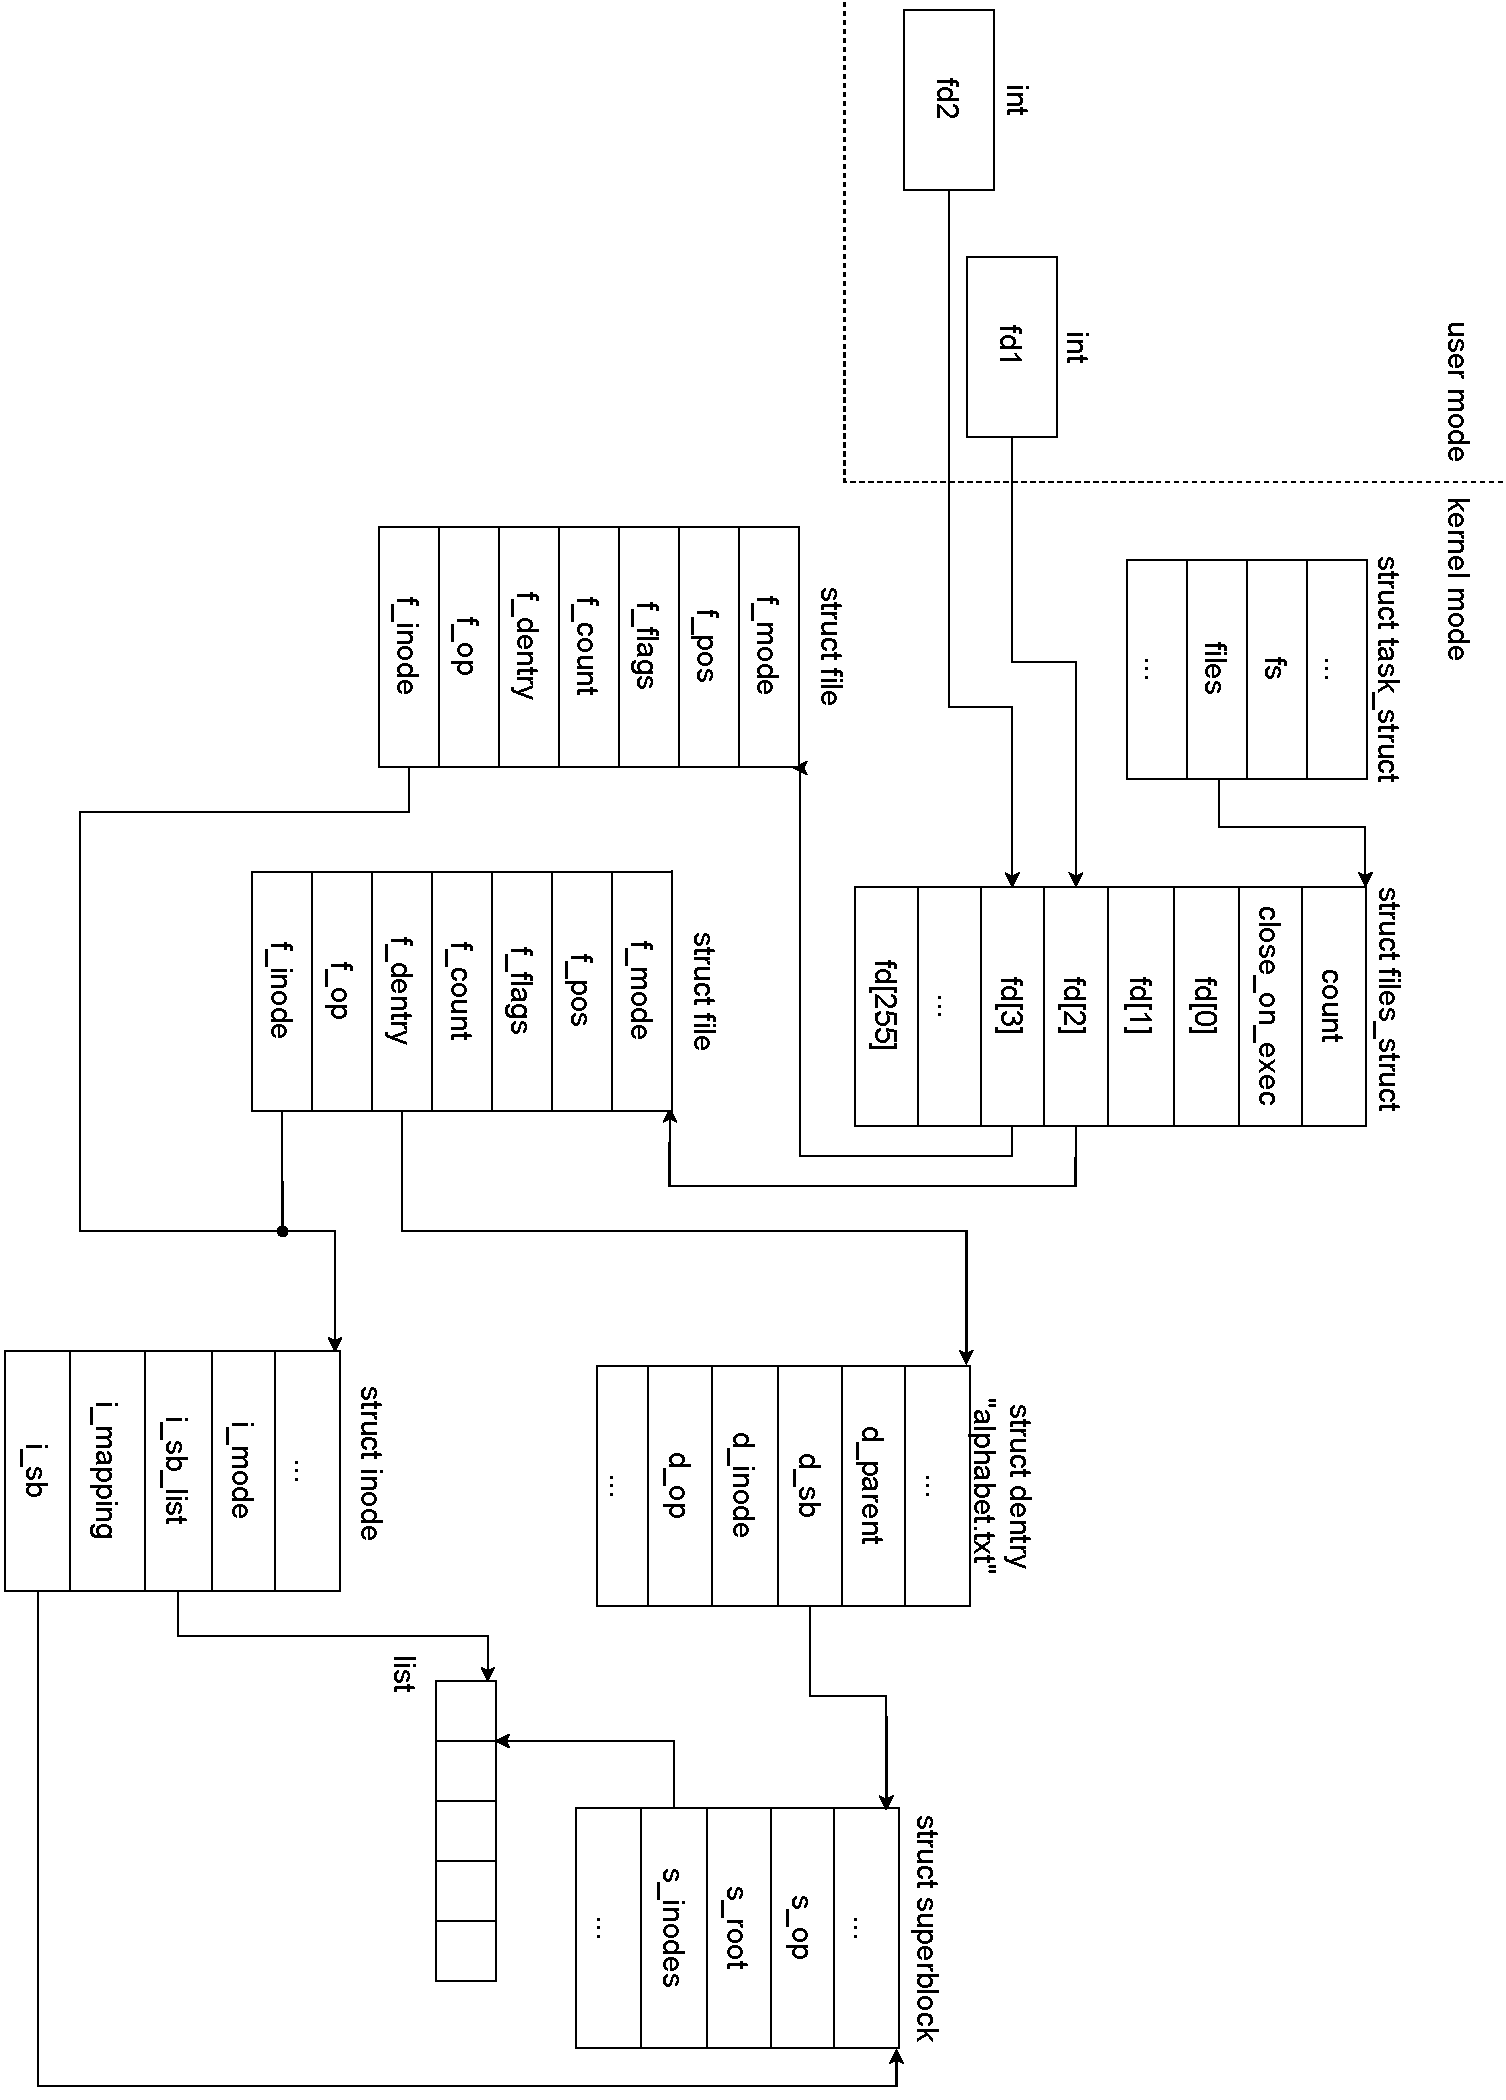
\includegraphics[width=150mm]{image/d2}
	\caption{Связи структур во второй программе}
\end{figure}

\newpage
\subsection{Многопоточный вариант}
\begin{code}
	\captionof{listing}{Вторая программа с созданием двух дополнительных потоков}
	\inputminted
	[
	frame=single,
	framerule=0.5pt,
	framesep=10pt,
	fontsize=\small,
	tabsize=4,
	linenos,
	numbersep=5pt,
	xleftmargin=10pt,
	]
	{c}
	{code/2_2.c}
\end{code}

\begin{figure}[!hbpt]
	\centering
	
\includegraphics[width=\textwidth]{image/2-2}
	\caption{Вывод программы}
\end{figure}


В однопоточной программе в цикле каждый символ из файла выводится два раза подряд, а в многопоточной программе порядок вывода символов не определён, так как потоки выполняются параллельно. При этом дополнительный поток начинает вывод позже главного, так как затрачивается время на его создание.

При создании дополнительных потоков связи структур не изменяются, так как ресурсами (в том числе и открытыми файлами) владеет процесс.

\newpage
\section{Вторая программа, второй вариант}

\subsection{Базовый вариант}
\begin{code}
	\captionof{listing}{Вторая программа, второй вариант, базовый вариант}
	\inputminted
	[
	frame=single,
	framerule=0.5pt,
	framesep=10pt,
	fontsize=\small,
	tabsize=4,
	linenos,
	numbersep=5pt,
	xleftmargin=10pt,
	]
	{c}
	{code/22_1.c}
\end{code}

\begin{figure}[h]
	\centering
	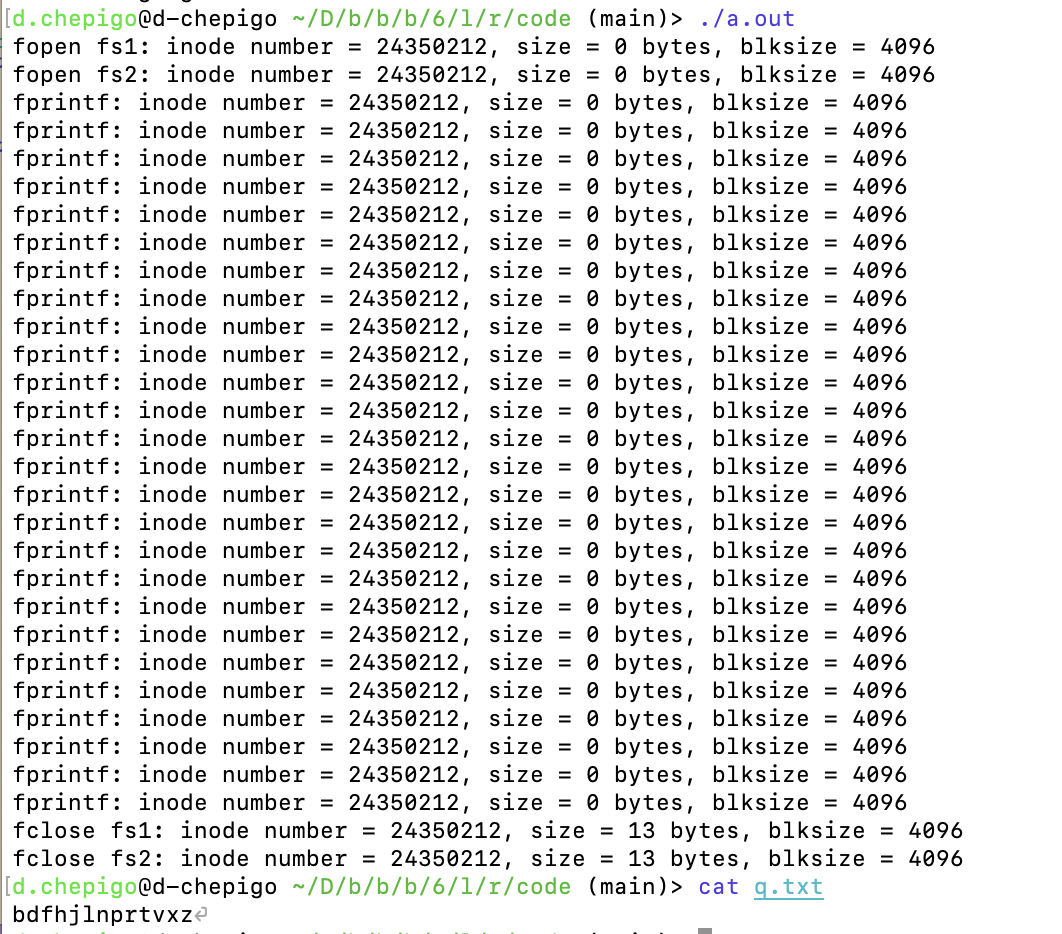
\includegraphics[width=\textwidth]{image/22-1}
	\caption{Вывод программы}
\end{figure}

В программе файл дважды открывается на запись функцией fopen() из библиотеки stdio.h. В системной таблице открытых файлов создаётся два дескриптора struct file, каждый из которых имеет собственный указатель f\_pos, но оба ссылаются на один и тот же inode. С помощью библиотечной функции fprintf() выполняется буферизованный вывод. Буфер создается без явного указания. Существует 3 причины, по которым данные из буфера записываются в файл:

\begin{enumerate}[label*=\arabic*.]
	\item Буфер заполнен.
	\item Вызвана функция fflush() --- принудительная запись.
	\item Вызвана функция close()/fclose().
\end{enumerate}

В данном случае запись в файл происходит в результате вызова функции fclose(). При вызове fclose() для fs1 буфер для fs1 записывается в файл. При вызове fclose() для fs2, все содержимое файла очищается, а в файл записывается содержимое буфера для fs2. В итоге произошла потеря данных, в файле окажется только содержимое буфера для fs2.



\newpage
\subsection{Связи структур}
\begin{figure}[!h]
	\centering
	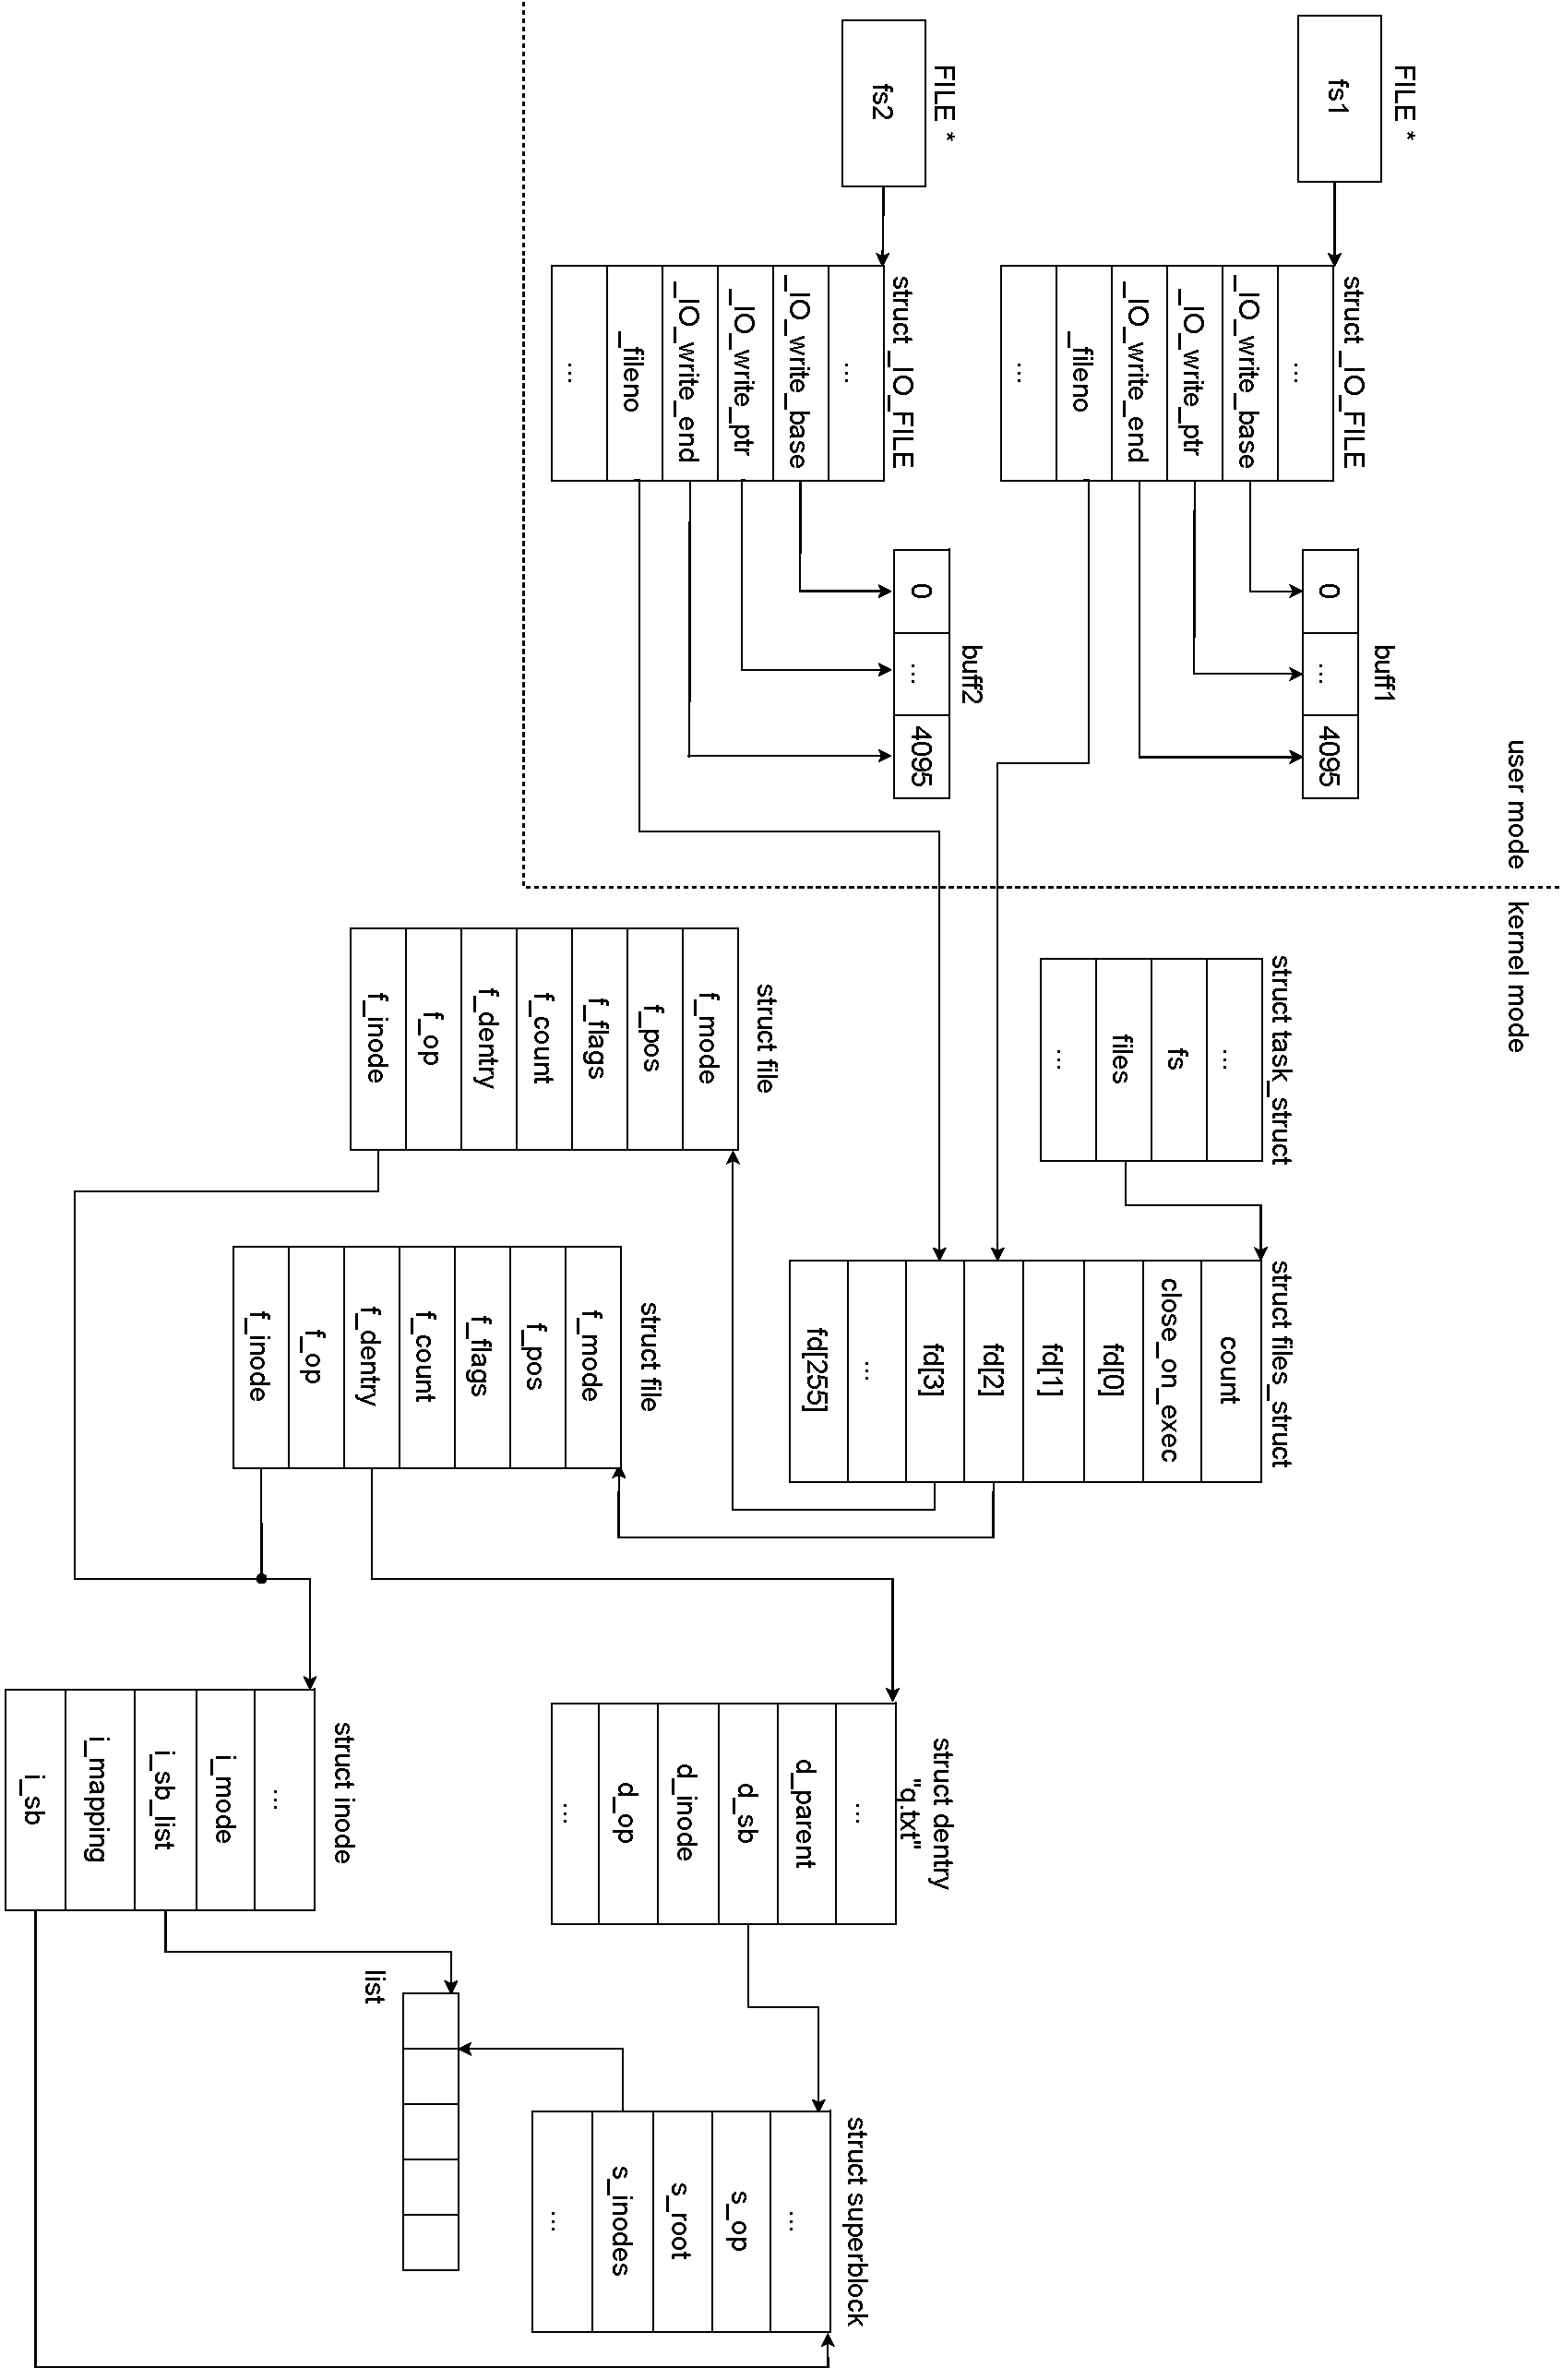
\includegraphics[width=150mm]{image/d3}
	\caption{Связи структур во втором варианте второй программы}
\end{figure}

\newpage

\subsection{Многопоточный вариант}
\begin{code}
	\captionof{listing}{Второй вариант второй программы с созданием двух дополнительных потоков}
	\inputminted
	[
	frame=single,
	framerule=0.5pt,
	framesep=10pt,
	fontsize=\small,
	tabsize=4,
	linenos,
	numbersep=5pt,
	xleftmargin=10pt,
	]
	{c}
	{code/22_2.c}
\end{code}

\clearpage

\begin{figure}[h]
	\centering
	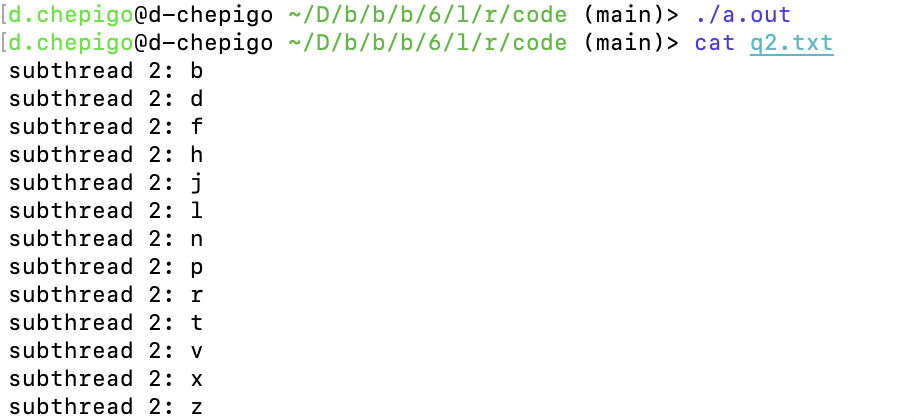
\includegraphics[width=\textwidth]{image/22-2}
	\caption{Вывод программы}
\end{figure}

В многопоточной программе работа с файлом производится аналогично однопоточной программе. Если вызывать fclose() в дополнительном потоке, то порядок вывода символов будет не определён, так как нельзя предсказать заранее, какой поток последним вызовет fclose().

При создании дополнительных потоков связи структур не изменяются, так как ресурсами (в том числе и открытыми файлами) владеет процесс.
